\InputIfFileExists{../data/global.tex}\relax\relax

\iffull
\setbox\pinguA=\hbox{\tikz\marmot[whiskers=gray];}\relax
\titlesuffix{\tikzpicture[@O]
    \node[above left,yshift=\btdmfootheight] at(current page.south east) {\copy\pinguA};
\endtikzpicture}

\title{Täglich grüßt das Murmeltier!} % \ldots\ sich selbst
\subtitle{Tutorium sieben}
\date{KW 25}
\addbibresource{references.bib}
\fi
\SetTutoriumNumber{7}

\iffull\begin{document}
\titleframe

\TopicOverview{7}
\fi

\iffull{\SummaryFrame
\begin{frame}[c]{Kurzwiederholung}
\begin{itemize}[<+(1)->]
   \itemsep14pt
    \item Eine Methode die sich selbst aufruft heißt rekursiv \begin{itemize}
    \item Die Rekursion ist linear, wenn sie sich maximal einmal selbst aufruft
    \item Solche sind \say{End-Rekursiv}, wenn der Aufruf das letzte ausgeführte Statement ist
    \item Rekursion und Iteration sind dabei gleichmächtig
   \end{itemize}
   \item Damit wir Bezeichner verwenden können müssen diese gültig und sichtbar sein \begin{itemize}
        \item Die Gültigkeit hängt an der Deklaration (Überschattung,~\ldots)
        \item Die Sichtbarkeit hängt an Modifikatoren wie \bjava{public}, \bjava{private},~\ldots
   \end{itemize}
   \item Methoden haben Seiteneffekte, wenn sie den Programmzustand über den Rückgabewert hinaus verändern
   \begin{itemize}
    \item Seiteneffekte sind ein großes Problem und sollten erstmal vermieden werden
    \item Ganz ohne geht es allerdings nicht (Konsolenausgaben,~\ldots)
   \end{itemize}
\end{itemize}
\end{frame}
}\fi

% TODO: make sectionlink auto triggerat start of section
\SetNextSectionText[.6\linewidth]{I have learned more from my failures than can ever be revealed in the cold print of a scientific article. [\ldots] [Failures] are much more fun to hear about afterwards; they are not so funny at the time.\\---~C.~A.~R. Hoare~\cite{hoare20211980}}
\section{Präsenzaufgabe}
{\taskenum
\begin{frame}[fragile,c]{Präsenzaufgabe}
\begin{aufgabe}{Irgendwo sind meine Socken doch}
\task<2->{In der Vorlesung wurde der Binary Algorithmus zur Suche in einer geordneten Struktur vorgestellt. \begin{enumerate}[<+(1)->]
    \item Geben Sie an, wie das folgende Array vom Suchalgorithmus Binary Search nach dem Schlüssel \say{4} durchsucht wird.\onslide<3->{
    \begin{center}
        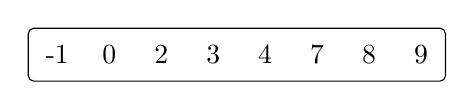
\begin{tikzpicture}
            \foreach[count=\i from 0] \a in {-1,0,2,3,4,7,8,9} {
                \node[outer sep=3pt] (\a) at (.66*\i, 0) {\a};
            }
            \draw[rounded corners=2pt] (-1.south west) rectangle (9.north east);
        \end{tikzpicture}
    \end{center}}
    \item<4-> Begründen Sie \textit{kurz}, weshalb der Binary Search Algorithmus eine worst-case Laufzeit von \(T(n)_{max} \in \O(\log n)\) hat.
\end{enumerate}}
\end{aufgabe}
\end{frame}
}

{
\iffull
\def\HandoutA{1}\def\HandoutB{2}\def\HandoutC{3}
\else
\def\HandoutA{1}\def\HandoutB{1}\def\HandoutC{1}
\fi
\begin{frame}[c]{Ja wie suchen wir denn die 4?}
\begin{center}
    \onslide<2->{\begin{tikzpicture}
        \foreach[count=\i from 0] \a/\ao/\ho/\co in {-1/2/0/{6-|handout:\HandoutB-},0/2/0/{6-|handout:\HandoutB-},2/2/0/{6-|handout:\HandoutB-},3/{2,3,4,5}/\HandoutA/{6-|handout:\HandoutB-},4/{2,3,9,10}/\HandoutC/{0|handout:0},7/{2,6,7,8}/\HandoutB/{9-|handout:\HandoutC-},8/{2,6}/0/{9-|handout:\HandoutC-},9/2/0/{9-|handout:\HandoutC-}} {
            \color{gray}\only<\ao|handout:\ho>{\color{black}}
            \expandafter\only\expandafter<\co>{\color{codeouthl}}
            \node[outer sep=3pt] (\a) at (.66*\i, 0) {\a};
            \node[below=2mm,codeouthl,font=\footnotesize\sffamily] (\a-i) at(\a.south) {\i};
        }
        \draw[rounded corners=2pt] (-1.south west) rectangle (9.north east);
        \onslide<3|handout:0>{\path(3-i.north)--(4-i.north) coordinate[pos=.5] (@); \node[above=-2mm] at(@.north) {\faAngleUp};}
        \onslide<4-5|handout:\HandoutA>{\node[above=-2mm] at(3-i.north) {\faAngleUp};}
        \onslide<5|handout:\HandoutA>{\node[above=2mm] at(3.north) {\(3 < 4\)};}
        \onslide<6|handout:0>{\path(7-i.north)--(8-i.north) coordinate[pos=.5] (@); \node[above=-2mm] at(@.north) {\faAngleUp};}
        \onslide<7-8|handout:\HandoutB>{\node[above=-2mm] at(7-i.north) {\faAngleUp};}
        \onslide<8|handout:\HandoutB>{\node[above=2mm] at(7.north) {\(7 > 4\)};}
        \onslide<9-10|handout:\HandoutC>{\node[above=-2mm] at(4-i.north) {\faAngleUp};}
        \iffull\onslide<10|handout:\HandoutC>{\node[above=2mm] at(4.north) {\(4 = 4\)};}\fi
    \end{tikzpicture}}
\end{center}
\begin{enumerate}
    \itemsep7pt
    \setcounter{enumi}{-1}
    \item<2-|handout:\HandoutA-> Initial ist \(\text{min = 0}\) und \(\text{max = 7}\). Wir springen in die Mitte: \(\text{mid} = \floor{(\text{min} + \text{max})/2}\). \onslide<4->{\infoblock{Hierbei runden wir im Gleichheitsfall ab. Das ist an sich willkürlich, hier aber von uns festgesetzt.}}
    \item<5-|handout:\HandoutA-> Das betrachtete Element ist kleiner als der Schlüssel, wir springen in die rechte Hälfte.\onslide<6->{\infoblock{Das heißt wir verschieben \(\text{min} = \text{mid} + 1\) und wiederholen die Berechnung von \(\text{mid}\).}}
    \item<8-|handout:\HandoutB-> Das betrachtete Element ist größer als der Schlüssel, wir springen in die linke Hälfte. \infoblock{Das heißt wir setzen \(\text{max} = \text{mid} - 1\) und wiederholen die Berechnung von \(\text{mid}\).}
    \item<10-|handout:\HandoutC> Das betrachtete Element entspricht dem gesuchten, liefere Index: \(4\) zurück.
\end{enumerate}
\begin{tikzpicture}[@O]
    \node[below left,yshift=-1.35cm,align=left] at(current page.north east) {\only<3-|handout:\HandoutA->{\(\frac{0+7}{2} = 3.5 \onslide<4->{\rightarrow 3}\)}\\[1.5mm]\only<6-|handout:\HandoutB->{\(\frac{4+7}{2} = 5.5 \onslide<7->{\rightarrow 5}\)}};
\end{tikzpicture}
\end{frame}
}

\begin{frame}{Und warum ist das schnell?}
    \begin{itemize}[<+(1)->]
        \itemsep10pt
        \item Mit jedem Vergleich sind wir entweder fertig, oder wir halbieren den Suchraum
        \item Bei \(n\) Elementen können wir maximal \(\log_2(n)\) oft halbieren \infoblock{Ist \(n = 8\) so beispielsweise \(\log_2(8) = 3\) mal.}
        \item So benötigen wir maximal \(\log_2(n)\) viele Vergleichsschritte
        \item Bei der \(\O\)-Notation ist die Basis des Logarithmus egal\infoblock{So ist für \(\log_a(x)\) der Unterschied zu \(\log_b(x)\) nur ein Faktor, der sich durch den Basiswechsel ergibt. Es ist: \(\log_a(x) = \frac{\log_b(x)}{\log_b(a)}\) dabei ist \(\log_b(a)\) eine Konstante die von der \(\O\)-Notation verschluckt wird.}
        \item Alle anderen Operationen benötigen konstante Zeit \info{sie sind nicht von \(n\) abhängig}
        \item So kommen wir auf \(\O(\log n)\)
    \end{itemize}
\end{frame}

\SetNextSectionText{Grundlagen der Rekursion\\Abgabe: \DTMDate{2022-06-20}}
\section{Übungsblatt 7}
\subsection{Aufgabe 1}
{\taskenum
\begin{frame}[fragile,c]{Aufgabe 1: Ablauf eines rekursiven Programms}
    \task<2->{Für einen rekursiv definierten Algorithmus kann man ein \say{Berechnungsformular} aufstellen, das für jeden rekursiven
    Aufruf (Inkarnation) vervielfältigt wird. Das Ergebnis der Berechnung wird dann durch Ein- und Rückübertragung
    von (Teil-) Lösungen bestimmt, wobei die Termination durch die Reduktion des Arguments ausgelöst wird. In dieser
    Aufgabe sollen Sie eine derartige Formularmaschine selbst angeben.\medskip

    \onslide<3->{Betrachten Sie das folgende rekursive Programm und geben Sie das Formularblatt, sowie die Inkarnationen für den Aufruf \T{ggt(6, 3)} an. Folgen Sie dabei der Gestaltung und Ausführung des Beispiels aus der Vorlesung (Kap.~8, Folien 15ff.)}}
    \begin{plainjava}
!*\onslide<4->*!public int ggT(int a, int b) {
!*\onslide<4->*!    if(b == 0) {
!*\onslide<4->*!        return a;
!*\onslide<4->*!    } else {
!*\onslide<4->*!        return ggt(b, a % b);
!*\onslide<4->*!    }
!*\onslide<4->*!}
    \end{plainjava}
\end{frame}
}

\begin{frame}[b,fragile]{Formulargefahr}
\forestset{K/.style={for tree={inner sep=4pt,block,minimum width=2em,outer sep=0pt,execute at begin node={\strut},grow=north,s sep=1.45em,l sep=1.5em}}}
\tikzset{every label/.style={gray},label distance=-.5mm,every path/.append style={line cap=round}}
\begin{tikzpicture}[@O]
\begin{onlyenv}<2->
\node[below left,yshift=-1.35cm,text width=4.5cm] at(current page.north east) {\lstfs{7}\begin{plainjava}
public int ggT(int a, int b) {
    if(b == 0) {
        return a;
    } else {
        return ggt(b, a % b);
    }
}
    \end{plainjava}};
\end{onlyenv}
\onslide<0|handout:1->{\node[above left,yshift=\btdmfootheight,T,text width=4cm] at(current page.south east) {Das Abschneiden von Ästen hier durch ausgrauen!};}
\end{tikzpicture}%\vspace*{-1.5\baselineskip}
\begin{onlyenv}<3-|handout:1->
\raisebox{-.5\height}{\begin{forest} K
   [\only<3-17|handout:-2>{{\paletteA{\faQuestion}}}\only<18-|handout:3->{\bfseries3},label=left:\strut ggT[3,label=right:\strut b][6,label=left:\strut a]]
   \node[above right] at(current bounding box.north west) {Initialer Aufruf};
   \pgfonlayer{background}
   \draw[thick,rounded corners=2pt] ([xshift=-2.15mm,yshift=-2mm]current bounding box.south west) rectangle ([xshift=2mm,yshift=2mm]current bounding box.north east);
   \endpgfonlayer
\end{forest}}\onslide<4->{\quad$\equiv$\quad\raisebox{-.5\height}{\colorlet{@@}{black}\only<7->{\colorlet{@@}{codeouthl}}\begin{forest} K
    % TODO: do the 0 6 false thingy first, and do not evaluate the b = 3 stuff in the then case, be consistent!
    % phantom to get the crap out of that
    [\only<11-16|handout:-2>{{\color{codeouthl}?}}\only<17-|handout:3->{\bfseries3},label=left:\strut if[\only<11-16|handout:-2>{\paletteA{\faQuestion}}\only<17-|handout:3->{\paletteA{\bfseries3}},label=right:\strut ggT,edge label={node[midway,right]{\footnotesize else}}[\only<9->{0},label=left:\strut \%[\only<8->{3},label=right:\strut b][\only<8->{6},label=left:\strut a]][\only<10->{3},label=above:b]][\only<7->{6},@@,label=above:a, edge label={node[pos=.55,left,align=right]{\footnotesize th\rlap{-}\\[-2.5mm]\footnotesize en}},edge=@@][\phantom{false}\only<6->{\llap{false}},label=left:\strut {=}, edge label={node[midway,left]{\footnotesize when}}[0][\only<5->{3},label=above:b]]]
    \node[above right] at(current bounding box.north west) {Inkarnation \(1\): \(a = 6\), \(b = 3\)};
    \pgfonlayer{background}
    \draw[thick,rounded corners=2pt] ([xshift=-2mm,yshift=-2mm]current bounding box.south west) rectangle ([xshift=4.25mm,yshift=2mm]current bounding box.north east);
    \endpgfonlayer
    % \node[below] at(current bounding box.south) {\smash{\T{ggt(6,3)}}};
    % TODO:animationen von unten ncach oben und andere steps mit handout breakds, bei der zwei einfach nur sperat animieren wie die aufploppenund bei der drei mehr reden als auf die FOlien packen (vielleicht einn QR code zum numberphile video oder so....)
 \end{forest}}}%
 \onslide<11-16|handout:2>{\qquad\llap{\raisebox{-.6\height}{\colorlet{@@}{black}\only<14->{\colorlet{@@}{codeouthl}}\begin{forest} K
    % TODO: do the 0 6 false thingy first, and do not evaluate the b = 3 stuff in the then case, be consistent!
    % phantom to get the crap out of that
    [\only<16->{3},label=left:\strut if[{},for tree={@@,edge=@@},label=right:\strut ggT,edge label={node[midway,right]{\footnotesize else}}[{},label=left:\strut \%[0,label=right:\strut b][3,label=left:\strut a]][0,label=above:b]][\only<15->{3},label=above:a, edge label={node[pos=.55,left,align=right]{\footnotesize th\rlap{-}\\[-2.5mm]\footnotesize en}}][\phantom{true}\only<13->{\llap{true}},label=left:\strut {=}, edge label={node[midway,left]{\footnotesize when}}[0][\only<12->{0},label=above:b]]]
    \node[above right] at(current bounding box.north west) {Inkarnation \(2\): \(a = 3\), \(b = 0\)};
    \pgfonlayer{background}
    \draw[thick,fill=btdm@background,rounded corners=2pt,fill opacity=.885] ([xshift=-2mm,yshift=-2mm]current bounding box.south west) rectangle ([xshift=4.25mm,yshift=2mm]current bounding box.north east);
    \endpgfonlayer
    % \node[below] at(current bounding box.south) {\smash{\T{ggt(3,0)}}};
 \end{forest}}}}
\end{onlyenv}
\end{frame}

\subsection{Aufgabe 2}
\begin{frame}[c]{Aufgabe 2: Rekursive Algorithmen implementieren}
    \task<2->{Unter dem Integral \(R \das \int_a^b f(x) \dif x\) einer Funktion \(f\) versteht man auch die Fläche zwischen der \(x\)-Achse und dem Graphen der Funktion. Im Folgenden sollen Sie eine rekursive Approximation \(A(a, b)\) für das Integral der Funktion \(f(x) = x^2\) im Intervall \([a, b]\) implementieren. Dazu sollen Sie das Intervall solange in Teilintervalle halbieren, bs diese für eine direkte Berechnung hinreichend klein sind. Anschließend werden alle Teilflächen addiert. Es ergibt sich also folgende Rekursionsgleichung: \onslide<3->{\begin{equation*}
        A^t(a, b) \das \begin{cases}
            (b - a) \cdot f(a) & \text{ falls } b - a \leq 0.01 \\
            A^{t + 1}\bigl(a, (a + b) / 2\bigr) + A^{t + 2}\bigl((a + b)/2, b\bigr),& \text{ sonst }
        \end{cases}
    \end{equation*}}
    \onslide<4->{Implementieren Sie eine Methode, die das Integral wie beschreiben rekursiv approximiert und das Ergebnis als Resultat zurückgibt. Testen Sie Ihre Implementierung für das Intervall \([0, 1]\).}}
\end{frame}

\begin{frame}[c,fragile]{Mathematische Definitionen übernehmen}
% no bold on handout
\def\M#1#2{\rlap{$\only<#1>{\color{paletteA}\mathbf}{#2}$}\phantom{\only<handout:0>{\mathbf}{#2}}}
\onslide<2->{\begin{tikzpicture}[@O]
    \color{gray}
    \only<1-|handout:0>{\color{codeouthl}}
    \node[below left,xshift=-2mm,yshift=-1.25cm,text width=12cm,scale=.65] at(current page.north east) {\begin{align*}
        \only<4-5,10-|handout:0>{\color{gray}}f(x) &\only<4-5,10-|handout:0>{\color{gray}}= x^2\\
        \only<6-|handout:0>{\color{gray}}A^t(a, b) &\only<6-|handout:0>{\color{gray}}= \begin{cases}
            \M{8|handout:0}{(b - a) \cdot f(a)} & \text{ falls } \M{7|handout:0}{b - a \leq 0.01} \\
            \M{9|handout:0}{A^{t + 1}\bigl(a, (a + b) / 2\bigr) + A^{t + 2}\bigl((a + b)/2, b\bigr)},& \M{7|handout:0}{\text{ sonst }}
    \end{cases}
\end{align*}};
\end{tikzpicture}}\vspace*{-\baselineskip}
\begin{plainjava}[add to literate={∫}{{$\int$}}1]
!*\CodeFileMarkerAttach<3->{Rekursion.java}*!
!*\onslide<2->*!public class Rekursion {
!*\onslide<4->*!   public static double f(double x) {
!*\onslide<5->*!      return x * x;
!*\onslide<4->*!   }!*\medskip*!
!*\onslide<6->*!   public static double A(double a, double b) {
!*\onslide<7->*!      if(b - a <= 0.01)
!*\onslide<8->*!         return (b - a) * f(a);
!*\onslide<7->*!      else
!*\onslide<9->*!         return A(a, (a + b)/2) + A((a + b)/2, b);
!*\onslide<6->*!   }!*\medskip*!
!*\onslide<10->*!   public static void main(String[] args) {
!*\onslide<11->*!      System.out.println("∫[0,1] x^2 = " + A(0,1));
!*\onslide<10->*!   }
!*\onslide<2->*!}!*\onslide<1->*!
\end{plainjava}
\end{frame}

\subsection{Aufgabe 3}
{\taskenum
\begin{frame}[c]{Aufgabe 3: Nicht-monotone Rekursion}
    \task<2->{Die bisher in der Vorlesung betrachteten rekursiven Algorithmen haben alle eine monoton in der Argumentgröße steigende Laufzeit. Es gibt aber rekursive Funktionen, bei denen diese Annahme nicht zutrifft. Ein Beispiel hierfür ist die \hlink{https://de.wikipedia.org/wiki/Collatz-Problem}{Collatz Funktion}, die für \(n \geq 1\) wie folgt definiert sei: \onslide<3->{\begin{equation*}
        C(n) \das \begin{cases}
            1 & \text{ falls } n = 1 \\
            C(n/2) & \text{ falls } n \text{  gerade} \\
            C(3n + 1) & \text{ sonst}
        \end{cases}
    \end{equation*}}
    \begin{enumerate}
        \item<4-> Implementieren Sie die Collatz Funktion in Java, messen Sie jeweils die Ausführungszeit in Nanosekunden (s. \T{System.nanoTime()}) für die Eingaben von \(1\) bis \(1000\) und lassen Sie sich diese ausgeben.
        \item<5-> Was können Sie über den Zusammenhang von \(n\) und der Ausführungszeit sagen? Schreiben Sie Ihre Antwort als Kommentar in die Java Datei.
    \end{enumerate}}
\end{frame}
}

\begin{frame}[c,fragile]{Ein wenig mehr von Collatz}
\def\M#1#2{\rlap{$\only<#1>{\color{paletteA}\mathbf}{#2}$}\phantom{\only<handout:0>{\mathbf}{#2}}}
\onslide<2->{\begin{tikzpicture}[@O]
    \color{gray}
    \node[below left,xshift=-2mm,yshift=-1.25cm,text width=12cm,scale=.65] at(current page.north east) {\begin{equation*}
        C(n) = \begin{cases}
            \M{6|handout:0}{1} & \M{4|handout:0}{\text{ falls }} \M{5|handout:0}{n = 1} \\
            \M{8|handout:0}{C(n/2)} & \M{4|handout:0}{\text{ falls }} \M{7|handout:0}{n \text{  gerade}} \\
            \M{9|handout:0}{C(3n + 1)} & \M{4|handout:0}{\text{ sonst}}
        \end{cases}
\end{equation*}};
\end{tikzpicture}}\vspace*{-\baselineskip}
\begin{plainjava}
!*\CodeFileMarkerAttach<3->{Collatz.java}*!
!*\onslide<2->*!public class Collatz {
!*\onslide<3->*!   public static int C(int n) {
!*\onslide<4->*!      if !*\onslide<5->*!(n == 1)
!*\onslide<6->*!         return 1;
!*\onslide<4->*!      else if !*\onslide<7->*!(n % 2 == 0)
!*\onslide<8->*!         return C(n / 2);
!*\onslide<4->*!      else
!*\onslide<9->*!         return C(3 * n + 1);
!*\onslide<3->*!   }

!*\onslide<2->*!}!*\onslide<1->*!
\end{plainjava}
\begin{onlyenv}<10->
\begin{tikzpicture}[@O]
    \node[above left,yshift=\btdmfootheight,text width=9.75cm,outer sep=0pt] (@) at(current page.south east) {%
\begin{plainjava}
!*\onslide<10->*!   public static void main(String[] args) {
!*\onslide<11->*!      for (int i = 1; i <= 1_000; i++) {
!*\onslide<12->*!         long start = System.nanoTime();
!*\onslide<13->*!         C(i);
!*\onslide<14->*!         System.out.println("C(" + i + ") = "
!*\onslide<14->*!            + (System.nanoTime() - start));
!*\onslide<11->*!      }
!*\onslide<10->*!   }!*\onslide<1->*!
\end{plainjava}
    };
    \draw[gray,decorate,decoration={brace,mirror,amplitude=5pt}] ([xshift=5mm,yshift=-3mm]@.north west) -- ([xshift=5mm,yshift=3mm]@.south west);
\end{tikzpicture}
\end{onlyenv}
\end{frame}

\iffull
{\pgfplotsset{K/.style={width=.95\linewidth,height=\textheight,scaled ticks=false,xlabel=$i$,xticklabel style={align=center,font=\footnotesize,execute at begin node=\vphantom{1234567890}},legend pos=north west,legend style={nodes={font=\small,align=left},draw=none,rounded corners=1.25pt},legend cell align={left},bar width=.18pt,ymin=0,ymajorgrids,ylabel={Time [\si{\nano\second}]},xlabel={\scriptsize i (for $C(i)$)},major tick length=0pt,axis lines=left,xmin=-1,enlarge x limits={abs=1ex,upper},enlarge y limits={abs=1ex,upper},extra y ticks={#1},extra y tick style={paletteD,font=\footnotesize,grid=major,grid style={paletteD,thick}}, ytickmin=2,,legend columns=2,legend style={/tikz/column 2/.style={column sep=5pt}},axis line style={-Kite,line join=round,line cap=round},legend image post style={rounded corners=1.25pt},ylabel near ticks,xlabel near ticks,xlabel shift=5mm}}
\begin{frame}[b]
\null\vspace*{1em}
\begin{onlyenv}<2|handout:1>
\begin{tikzpicture}
    \begin{axis}[K={402.873}]% avg
        \addplot[ybar,fill,paletteA!80!lightgray] table[x=i,y=time,col sep=comma] {logging.data};
    \end{axis}
\end{tikzpicture}
\end{onlyenv}%
\begin{onlyenv}<3|handout:2>
\begin{tikzpicture}
    \begin{axis}[K={88.4737184999999},ytick={50,200,300}]% avg
        \addplot[ybar,fill,paletteA!80!lightgray] table[x=i,y=time,col sep=comma] {logging-avg.data};
    \end{axis}
\end{tikzpicture}
\end{onlyenv}%
\begin{tikzpicture}[@O]
    \onslide<2|handout:1>{\node[below=2mm,T] at(current page.north) {Cherry-Picked, 1 Durchlauf (Teils bis \SI{30000}{\nano\second})};}
    \onslide<3|handout:2>{\node[below=2mm,T] at(current page.north) {Gemittelt über \num{100000} Läufe};}
\end{tikzpicture}
\end{frame}
\begin{frame}{Woher die Schwankungen}
\begin{itemize}[<+(1)->]
    \itemsep12pt
    \item Benchmarking ist eigentlich um einiges tückischer!\;\raisebox{-4pt}{\smash{\textsuperscript{\cite{microbenchmarks}}}} \begin{itemize}
        \item Das Zeitmessen selbst braucht Zeit
        \item Die Java Virtual Machine hat zu Beginn einiges zusätzlich zu tun
        \item Dienste wie die Garbage-Collection können unkontrolliert dazwischenfunken
    \end{itemize}
    \item Dafür gibt es Bibliotheken wie \hlink{https://github.com/openjdk/jmh}{jmh} oder \hlink{https://github.com/google/caliper}{caliper}
    \item Hier ging es uns aber auch nicht um die exakten Zeiten, sondern nur um seltsame Schwankungen \begin{itemize}
        \item Für die hätte man aber auch einfach die Rekursiontiefe aufzeichnen können
        \item Menno\ldots
    \end{itemize}
\end{itemize}
\end{frame}
}
\fi

\begin{frame}{Ausführungszeitzusammenhänge}
    \begin{itemize}[<+(1)->]
        \itemsep8pt
        \item Zwischen \(n\) und der Ausführungszeit existiert kein offensichtlicher Zusammenhang
        \item Ganz allgemein zeigt die Collatz-Funktion wie eine einfache Formulierung ein quasi unmöglich vorhersehbares Verhalten an den Tag legen kann\;\raisebox{-4pt}{\smash{\textsuperscript{\cite{van2005collatz}, \cite{andrei1998collatz}}}} \begin{itemize}
            \itemsep2pt
            \item $C(870)$ benötigt beispielsweise $28$ Schritte
            \item $C(871)$ benötigt hingegen $178$ Schritte
            \item $C(872)$ benötigt wieder $116$ Schritte
            \item $C(876)$ benötigt nur $54$ Schritte
            \iffull\item $C(14039)$ bedarf ebenfalls nur $45$ Schritte
            \item $C(9780657630)$ bedarf hingegen $1132$ Schritte
            \item $C(9780657633)$ wieder nur $248$ Schritte
            \fi
        \end{itemize}
    \end{itemize}
\end{frame}

\iffull
\SetNextSectionText{Suchen und Sortieren\\Abgabe: \DTMDate{2022-06-27}}
\section{Aussicht: Übungsblatt 8}
\subsection{Aufgabe 1}
\begin{frame}{Aufgabe 1: Naive Sortieralgorithmen}
\begin{itemize}[<+(1)->]
    \itemsep12pt
    \item Bei manchen Problemen kann gezeigt werden,\pause{} dass sie sich nicht besser lösen lassen.\pause{} So zum Beispiel das Sortierproblem,\pause{} welches immer mindestens in \(\O(n \log n)\) liegt (\emph{average-case}).\pause{} Man spricht auch von einer unteren Schranke.
    \item Ein paar Rechenregeln können hilfreich sein,\pause{} seien \(k, c\) Konstanten:\pause{}
    \begin{alignat*}{3}
        \onslide<9->{k} &\onslide<9->{= \O(1)} &\onslide<10->{ f(n)} &\onslide<10->{= \O(f(n))} \\
        \onslide<11->{c \cdot \O(f(n))} &\onslide<11->{= \O(f(n))}&\onslide<12->{ \O(f(n)) + \O(f(n))} &\onslide<12->{= \O(f(n))} \\
        \onslide<13->{\O(f(n)) \cdot \O(g(n))} &\onslide<13->{= \O(f(n) \cdot g(n))}\quad & \onslide<14->{\O(\O(f(n)))} &\onslide<14->{= \O(f(n))}
    \end{alignat*}
    \onslide<15->{Sowie: \onslide<16->{\(\O(f(n) + g(n)) = \O(\max\{f(n), g(n)\})\)}}
\end{itemize}
\end{frame}

\begin{frame}[t,fragile]{Die O-Notation}
\begin{itemize}[<+(1)->]
    \item Für die \(\O\)-Notation gilt \(T(n) \in \O(f(n))\), wenn \(f(n)\) eine obere Schranke von \(T(n)\) ist, also:\vspace*{-.125\baselineskip} \onslide<3->{\[T(n) \in \O(f(n))\pause{}\iff \exists n_0 \in \mathbb{N}\: c \in \mathbb{R}^+\: \forall n \geq n_0: T(n) \leq c \cdot f(n).\]\vspace*{-\baselineskip}}
    \item<4-> Neben den mathematischen Gesetzen (Logarithmus,~\ldots) reichen meist die folgenden:\vspace*{-.66\baselineskip}
\begin{center}%
\resizebox{\linewidth}{!}{%
\setlength{\aboverulesep}{0pt}%
\setlength{\belowrulesep}{0pt}%
\setlength{\extrarowheight}{.85ex}%
\begin{tabular}{c*{8}{c}}
    \toprule
    & \onslide<5->{\cellcolor{pingu@green!100!pingu@purple!21} \(\O(1)\)} & \onslide<6->{\cellcolor{pingu@green!85!pingu@purple!21}\(\O(\log n)\)} & \onslide<7->{\cellcolor{pingu@green!69!pingu@purple!21} \(\O(n)\)} & \onslide<8->{\cellcolor{pingu@green!53!pingu@purple!21} \(\O(n\log n)\)} & \onslide<9->{\cellcolor{pingu@green!36!pingu@purple!21} \(\O(n^2)\)} & \onslide<10->{\cellcolor{pingu@green!19!pingu@purple!21} \(\O(n^3)\)} & \onslide<11->{\cellcolor{pingu@green!14!pingu@purple!21} \(\O(2^n)\)} & \onslide<12->{\cellcolor{pingu@green!0!pingu@purple!21} \(\O(n!)\)} \\[0.45ex]\midrule
    Bsp: & \onslide<5->{\(42\)} & \onslide<6->{\(4 \log (3n)\)} & \onslide<7->{\(4n-3\)} & \onslide<8->{\(4n\log(2n)\)} & \onslide<9->{\(n^2 + 2n - 1\)} & \onslide<10->{\(n^3 - 42n^2\)} & \onslide<11->{\(14\cdot2^n\)}& \onslide<12->{\(n! \cdot 10^{-42}\)}\\
    Bez: &\onslide<5->{\footnotesize konst.} & \onslide<6->{\footnotesize logarithm.} & \onslide<7->{\footnotesize linear} &\onslide<8->{\footnotesize linear log.} & \onslide<9->{\footnotesize quadratisch} & \onslide<10->{\footnotesize kubisch} & \onslide<11->{\footnotesize exponentiell} & \onslide<12->{\footnotesize faktoriell} \\
\bottomrule
\end{tabular}}\bigskip
\end{center}
\item<13-> Es existieren auch noch andere Notationen, die uns zunächst egal sind
\end{itemize}
\end{frame}

\subsection{Aufgaben 2 und 3}
\begin{frame}{Aufgaben 2 und 3}
\begin{itemize}[<+(1)->]
    \itemsep12pt
    \item Bei Best- und Worst-case Analysen gilt es, Eingaben zu finden die die beste und schlechteste Laufzeit liefern
    \item So wie das Nachvollziehen von Algorithmen schwer ist, kann es schwer sein diese für einen Algorithmus zu finden \info{hier hilft Übung}
    \item Für die Transformation von Iteration zu Rekursion hilft ein Blick auf die Präsenzaufgabe letzter Woche
\end{itemize}
\end{frame}
\fi

\SetNextSectionText[.55\linewidth]{There are two ways of constructing a software design: One way is to make it so simple that there are obviously no deficiencies, and the other way is to make it so complicated that there are no obvious deficiencies. The first method is far more difficult.\\---~C.~A.~R. Hoare~\cite{hoare20211980}}
\section{Abschließendes}
{\SummaryFrame
\begin{frame}[t]{Zusammenfassend}
\pause \printBibCommand
\vfill\vfill % double fill for more fraction
\begin{itemize}[<+(1)->]
    \itemsep4pt
    \item Rekursion ist neben Iteration ein mächtiger Abstraktionsmechanismus \begin{itemize}
        \item Ein gleichmächtiger, um genau zu sein
        \item Es erlaubt beispielsweise die Umsetzung von Divide-And-Conquer-Verfahren
    \end{itemize}
    \item Neben der Formularmaschine gibt es viele andere \hlink{https://github.com/EagleoutIce/Episode-Recursion}{Visualisierungen} für Rekursion
    \item Selbst einfach aussehende Algorithmen können sehr schwer nachvollziehbar sein!
    \item Bei der Komplexitätsbetrachtung hilft die \(\O\)-Notation zum Vergleich \begin{itemize}
        \item \(T(n) \in \O(f(n))\pause{}\iff \exists n_0 \in \mathbb{N}\: c \in \mathbb{R}^+\: \forall n \geq n_0: T(n) \leq c \cdot f(n)\)
        \item \say{Der am stärksten wachsende Ausdruck}
    \end{itemize}
\end{itemize}
\end{frame}
}

\outro{\vskip9mm\centering \onslide<2->{\scalebox{1.42}{\begin{tikzpicture}
    \pingu[body type=legacy,name=pingu,right wing wave,eyes wink,left wing grab,height=10mm,blush,feet=sit];
    \draw[line cap=round]([xshift=.15mm]pingu-wing-right) to[bend right] ++(.1mm,1.1mm) -- ++(4.5mm,8.5mm) coordinate(@);
    \scope[rotate around=-18:(@)]
    \fill[pingu@yellow!80!pingu@red,rounded corners=1.5pt] (@) --++(1mm,0mm) --++(-1mm,.33mm) arc(270:630:4.325mm and 4.7mm) -- ++(-1mm,-.33mm) -- cycle;
    \draw[line cap=round,pingu@black,very thin] (@)++(-.35mm,.3mm) to[bend right=14] ++(.7mm,0);
    \endscope
    \draw[line cap=round](pingu-wing-right) to[bend right] ++(-.65mm,1.4mm) -- ++(-2mm,8mm) coordinate(@);
    \scope[rotate around=10:(@)]
    \fill[pingu@green,rounded corners=1.5pt] (@) --++(1mm,0mm) --++(-1mm,.33mm) arc(270:630:4.25mm and 5.133mm) -- ++(-1mm,-.33mm) -- cycle;
    % \fill[pingu@white,fill opacity=.6] (@)++(-3mm,7.15mm) ellipse[x radius=.39mm,y radius=.42mm];
    \draw[line cap=round,pingu@black,very thin] (@)++(-.35mm,.3mm) to[bend right=14] ++(.7mm,0);
    \endscope
    \draw[line cap=round]([xshift=.1mm]pingu-wing-right) to[bend right] ++(-.55mm,1.4mm) -- ++(-.25mm,11mm) coordinate(@);
    \scope[rotate around=4:(@)]
    \fill[pingu@blue,rounded corners=1.5pt] (@) --++(1mm,0mm) --++(-1mm,.33mm) arc(270:630:4.125mm and 4.9mm) -- ++(-1mm,-.33mm) -- cycle;
    % \fill[pingu@white,fill opacity=.6] (@)++(-3mm,6.75mm) ellipse[x radius=.39mm,y radius=.42mm];
    \draw[line cap=round,pingu@black,very thin] (@)++(-.35mm,.3mm) to[bend right=14] ++(.7mm,0);
    \endscope
    \draw[line cap=round]([xshift=.1mm]pingu-wing-right) to[bend right] ++(-.85mm,1.35mm) -- ++(-5mm,4.5mm) coordinate(@);
    \scope[rotate around=30:(@)]
    \fill[pingu@purple,rounded corners=1.5pt] (@) --++(1mm,0mm) --++(-1mm,.33mm) arc(270:630:3.525mm and 4.3mm) -- ++(-1mm,-.33mm) -- cycle;
    \draw[line cap=round,pingu@black,very thin] (@)++(-.35mm,.3mm) to[bend right=14] ++(.7mm,0);
    \endscope
\end{tikzpicture}}}}

\iffull\end{document}\fi
